\chapter{Fazit und Ausblick}
\label{chapter:fazit}

\section{Fazit}
\label{sec:fazit_ausblick:fazit}

Eine \ac{SaaS} Implementation in einer Gaia-X kompatiblen Cloud ist mit dem aktuellen Stand des Gaia-X Projekts zwar schon 
möglich, bringt allerdings noch einige Unvollständigkeiten mit.
Aufgrund von noch sehr unausgereiften Implemtierungen der Gaia-X Services ist der produktive Einsatz eines \ac{SaaS}
Modells noch nicht zu empfehlen. 
Zu viele Services, die die europäische Cloud ausmachen sollen, sind nur als Referenzarchitekturen vorzufinden.
In der Plusserver Open Cloud, die auf dem \acf{SCS} basiert, finden sich aktuell weitgehend \ac{IaaS} Services wieder.
Diese Services belaufen sich größtenteils auf schlichte OpenStack Services, eine Innovation bleibt aus.

Kubernetes stellt sich allerdings als attraktive Plattform zum Bereitstellen und Verwalten dieser Services heraus.
Eine Zukunft des Containerorchestrierungsframework im Gaia-X Umfeld ist durchaus vorstellbar und wird ebenfalls von \ac{SCS}
angestrebt \cite{scs}.

\section{Ausblick}
\label{sec:fazit_ausblick:fazit}

\begin{figure}[h]
  \centering
  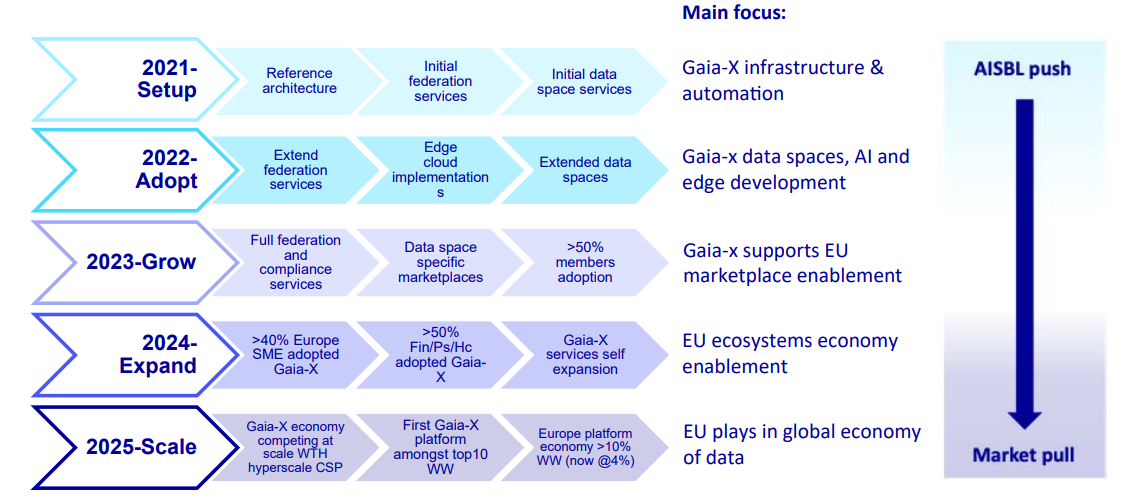
\includegraphics[width=1.1\textwidth]{gfx/chapters/6_fazit_ausblick/gaia-x-ausblick.png}
  \caption{Fünfjahresplan der Gaia-X Initiative}
  \label{fig:gaia-x-ausblick}
  \source{\cite{Bonfiglio2021}}
\end{figure}

Die Initiative Gaia-X befindet sich zur Zeit noch im Aufbau.
In \ref{fig:gaia-x-ausblick} wird der Fünfjahresplan der Initiative dargestellt.
Zum Zeitpunkt der Arbeit läuft die erste Phase: \emph{Setup}.
Eine Implementation der aufgeführten Referenzarchitektur exisitert allerdings noch nicht.

\citeauthor{Bonfiglio2021} strebt im genannten Fünfjahresplan eine vollständige Implementierung der Föderationsservices
im Jahr 2023 an.
Durch die Enstehung eines neuen Markts soll Gaia-X 2025, in der Phase \emph{Scale},
eine Konkurrenz für Hyperscaler Clouds im globalen Markt werden \cite{Bonfiglio2021}.



\section{Related Work}
\label{sec:fazit_ausblick:related_work}

In\cite{Truyen2016} beschreiben \citeauthor{Truyen2016}
das Erstellen von \emph{Multi-Tenant}
\acf{SaaS} mithilfe von Container Orchestrierungssoftware wie Kubernetes.
\acp{SaaS} werden immer häufiger auf skalierbaren Plattformen gehostet, um eine hohe Verfügbarkeit sowie Ausfallsicherheit zu gewährleisten.
Innerhalb ihres Papers gehen sie auf die Vor- und Nachteile des Containeransatzes ein.
Ein klarer Vorteil sei die Möglichkeit des Multi-Cloud Modells, da Kubernetes unabhängig der jeweiligen Cloud Anbieter einsetzbar ist.
und einen Standard implementieren.
Isolationsmöglichkeiten zwischen den \emph{Tenants} habe einen hohen Anspruch für Sicherheit und Datenschutz.
Ein weiterer Problemfall sei der hohe Aufwand zum Managment des Deployments\footnote{Bereitstellung} der Anwendung.
Sie präsentieren eine Referenzarchitektur zum Erstellen von Container basierten Multi-Tenant SaaSs.
Einen fehlenden Standard für Container Images bemängeln sie zum Zeitpunkt ihrer Veröffentlichung.
Als weiteren Verbesserungspunkt stellen \citeauthor{Truyen2016} 3 Möglichkeiten zur Isolation von Tenants vor.
Ein Einsatz des Kubernetes Operator Patterns, welche das Deployment der Anwendung an eine Komponente des \acf{SaaS} übergeben wird,
wurde in diesem Falle nicht beachtet. Das Operator Pattern wurde 2016 von CoreOS vorgestellt, wodurch zum Erscheinungszeitpunkt
des Papers dieses noch nicht vorhanden war.

\paragraph{}
Als weitere Möglichkeit zur Abstraktion von Softwaremanagment für Endnutzer entwickeln \citeauthor{Wieder2012} in ihrem Paper
\cite{Wieder2012} ein System, das die Cloud-Kunden von der Last befreit, zu entscheiden, welche Dienste innerhalb einer Cloud zu verwenden.
Dabei wird speziell auf den Fall von MapReduce Operationen eingegangen. Kunden sollen nur entsprechende Ziele definieren, beispielsweise
die Minimierung der Kosten, eine Berechnung, die in der Cloud ausgeführt werden soll, sowie eine Liste von Cloud Services.
Das System erstellt automatisch die Berechnung und optimiert während der Laufzeit die Anwendung basierend auf externen Zuständen.
Ein Problem liegt hierbei bei der Beschränkung auf kurzweilige Berechnungen, welche keine Grundlagen für \acp{SaaS} bieten.

\paragraph{}
Im Paper \cite{Bousselmi2014} wird das \ac{CPP} für SaaSs beschrieben, welches als Hauptziel die Optimierung der Ressourcennutzung
der Cloudkomponenten sowie die Minimerung der Antwortzeit verfolgt.
Eine gelungene Lösung für das \ac{CPP} solle folgende Anforderungen erfüllen:
\begin{itemize}
  \item \texttt{Platzierungsalgorithmus}
  \item \texttt{Infrastrukturbeschreibung}
  \item \texttt{Provisionierungsalgorithmus}
  \item \texttt{Cloudunabhängig}
\end{itemize}
Desweiteren bieten \citeauthor{Bousselmi2014} eine Übersicht der bereits existierenden Lösungen des \ac{CPP} für \acp{SaaS}.
Allerdings wurden nur das Nutzen von \acf{VM} bedacht, welche Nachteile gegenüber Container besitzen.
Da \acp{VM} zusätzlich Hardware virtualisieren müssen, wodurch Ressourcen eingespart werden können \cite{seo2014performance}.
Außerdem besitzen Container eine bessere Kosteneffizienz sowie Performance im Vergleich zu \acp{VM} \cite{soltesz2007container}.